\graphicspath{{Chapitre_6/Images/}}
\chapter{Model overview}\label{C6}
%%%%%%%%%%%%%%%%%%%%%%%%%%%%%%%%%%%
%%%%%                         %%%%%
%%%%% Introduction chapitre 5 %%%%%
%%%%%                         %%%%%
%%%%%%%%%%%%%%%%%%%%%%%%%%%%%%%%%%%
\quad\, In the chapter \ref{C5}, the Brayton cycle has been introduced by presenting two configurations. Also, it has been mentioned that many other configurations (illustrated in the annex \ref{annex:Brayton_variant}) exists to cover a large panel of applications. 

This chapter will be devoted to the description of the  Brayton cycle model. This model will only consider steady state operations. Thus, transient effects like the acceleration of the turbomachines or the heating up of the heat-exchangers will not be taken into consideration.
 

\section{Python language}
%%%%%%%%%%%%%%%%%%%%%%%%%%%%%%%%%%%
%%%%%                         %%%%%
%%%%%  <<Python language>>    %%%%%
%%%%%                         %%%%%
%%%%%%%%%%%%%%%%%%%%%%%%%%%%%%%%%%%
\quad\, Python is a computing language that was created by Guido van Rossum at the Centrum Wiskunde \& Informatica (CWI - \url{https://www.cwi.nl}) in the early 1990s. Starting 1995, G. van Rossum continued to work on Python at the Corporation for National Research Initiatives (CNRI - \url{https://www.cnri.reston.va.us/}). Since the very first release, the language was open source. This means that the source code was accessible to anyone. 

From this time, Python progressively gained in popularity, and the community participating in the development of the software didn't stop growing. Today, this language is used by many companies and for many types of applications. Indeed, this programming language is used for website creation, machine learning, automation, etc. 

Since Python is an open source language, it lives thanks to its community which creates and shares libraries. Indeed, what has already been implemented in the past can be freely used by the other users. Moreover, new users can easily start developing under Python thanks to huge amount of guide and documentation to starting learning about the Python language.

Also, Python is a programming language that allows the object-oriented programming. This paradigm consists in the definition of blocks of code (called objects) which are able to interact through relations, defined in order to solve a given problem. This allows creating computer code that can evolve through the times. 

\section{Model structure}
%%%%%%%%%%%%%%%%%%%%%%%%%%%%%%%%%%%
%%%%%                         %%%%%
%%%%% <<Structure of the>>    %%%%%
%%%%%      <<model>>          %%%%%
%%%%%                         %%%%%
%%%%%%%%%%%%%%%%%%%%%%%%%%%%%%%%%%%
\quad\, The focus of this section is the description of the structure of the computer code itself. The program is separated into multiple blocks which can interact between each other. Before explaining the role of each of these blocks, the global structure of the program will be given.

\subsection{Input file}
\quad\, To start the program, the user has to provide an input file that will contain all the required information to execute the program. The structure of the inputs follows the YAML scheme which is a language that allows storing data in a structure and readable ways for the human\footnote{YAML stands for \textbf{Y}AML \textbf{A}in't \textbf{M}arkup \textbf{L}anguage.} . The strength of such language is that any data can be expressed under an arbitrary name. 

When the python code read the file, the file will be interpreted as a nested dictionary. A dictionary in Python can be considered as a table that can contain elements of different types. In a nested dictionary, some of these elements are also dictionary.

Here the YAML file that is given to the program is composed of four dictionaries respectively identified by the names "Type", "Selection", "Input" and "Extra". An example of an input files is given in the appendix \ref{annex:yaml}. 

\subsubsection{Type}
\quad\ The dictionary "Type" is composed of only one field that specified which variant of the Brayton cycle is going to be studying. By specifying one of the names listed in the Table \ref{tab:C5_inputconfig}, the program will now the variant to load in the memory.

\subsubsection{Selection}
\quad\ Then, the second dictionary "Selection" is used to specialize the variant and is composed of boolean elements. The reading of this dictionary will say to the program what extra data are expected to be found in the dictionary ''Extra''.
\newpage
The first element "WHX" of this dictionary is about the choice to add a water heat exchanger to recover part of the temperature in the fumes. If the field is set to \textit{true}, the following inputs will be required:
\begin{itemize}
    \setstretch{1}
    \item $\varepsilon_{whx}$: Efficiency of the water heat exchanger (\%)
    \item $T_{whx,water,in}$, $T_{whx,water,out}$: Inlet and outlet temperature of the water (\degree C)
    \item $P_{whx,water, in}$: Inlet pressure of the water (\degree C)
    \item $Dp_{whx,water}$, $Dp_{whx,gas}$: Water and gas nominal pressure drops (\%)
\end{itemize}

Then, the field "MAP" gives the choice to use performance maps (provided by the user) for the compressor and the turbine. If set to \textit{true}, the absolute path to the performance maps and the rotational speed of the turbomachines have to be specified. The performance maps are given as Excel sheets where each row corresponds to an operating point characterized by \(\dot{m}_{corr}\), \(\Pi_{tt}\), \(N_{corr}\) and \(\eta_{is}\).

By default, the maps are not used. Instead, the following inputs are asked to be able to characterize the compressor and the turbine:

\begin{itemize}
\setstretch{1}
    \item $\eta_{is,c}$ and $\eta_{is,t}$: Isentropic efficiency of the compressor and the turbine (\%)
    \item $\Pi_{tt,c}$: Total to total compression ratio (-)
    \item $TIT$: Turbine Inlet Temperature (\degree C)
\end{itemize}

The parameter "VAR\_DP" included in the dictionary "Selection" is used to take into account the variation of the pressure drops with the mass flow rate. If this feature is desired, the nominal mass flow rate associated to the nominal pressure drop has to be specified.  

Similarly, the last parameter "Var\_EFF" in the dictionary allows taking into account the heat exchanger efficiency dependency to the temperature and mass flow rate of both flows. If this option is chosen, the nominal mass flow rate and the nominal inlet/outlet temperatures for which the heat exchanger has the specified efficiency are required.

\subsubsection{Input}
\quad\ This third dictionary contains all the default parameters that are required to assess the performance of the selected variant of the Brayton gas cycle. As an example, the Table \ref{tab:C6_inputRGT} includes the inputs that has to be specified.

\begin{longtable}[c]{@{}llc@{}}

\caption{Input - Regenerative Gas Turbine (RGT)}
\label{tab:C6_inputRGT}\\
\toprule
\textbf{Input}                        & \textbf{Abbreviation} & \textbf{Unit} \\* \midrule
\endfirsthead
%
\endhead
%
\bottomrule
\endfoot
%
\endlastfoot
%
Reference temperature                 & $T_{ref}$                                 & \degree C     \\
Reference pressure                    & $P_{ref}$                                 & Pa            \\
Ambient temperature                & $T_{amb}$                                 & \degree C     \\
Ambient pressure                      & $P_{amb}$                                 & Pa            \\
Fuel temperature                      & $T_{fuel}$                                & \degree C     \\
Mass flow rate of air                 & $\dot{m}_{air}$                           & kg/s          \\
Air factor                            & $\lambda$                                 & -             \\
\rowcolor[HTML]{FFFFC7} 
Compression ratio                     & $\Pi_{tt,c}$                              & -             \\
\rowcolor[HTML]{FFFFC7} 
Turbine Inlet Temperature             & $TIT$                                     & \degree C     \\
\rowcolor[HTML]{FFFFC7} 
Compressor isentropic efficiency      & $\eta_{is,c}$                             & \%            \\
\rowcolor[HTML]{FFFFC7} 
Turbine isentropic efficiency         & $\eta_{is,t}$                             & \%            \\
Combustion efficiency                 & $\eta_{cc}$                               & \%            \\
Shaft mechanical efficiency           & $\eta_{shaft}$                            & \%            \\
Generator efficiency                  & $\eta_{gen}$                              & \%            \\
Regenerator efficiency                & $\varepsilon_{re}$                        & \%            \\
Combustion chamber pressure drop      & $Dp_{cc}$                                 & \%            \\
Regenerator pressure drop (hot side)  & $Dp_{re,H}$                               & \%            \\
Regenerator pressure drop (cold side) & $Dp_{re,C}$                               & \%            \\
Duct pressure drop                    & $Dp_{duct}$                               & \%            \\
Chimney pressure losses               & $\Delta p_{chimney}$                      & Pa            \\
Fuel composition                      & $Fuel_{comp}$                             & -             \\
Air composition                       & $Air_{comp}$                              & -             \\* \bottomrule
\end{longtable}

The inputs emphasized in yellow in the Table \ref{tab:C6_inputRGT} are ones that are not used if the map of the compressor and the turbine are used. The air factor $\lambda$ is used to initiate the iterative search of the mass flow rate of fuel in the program. Any value greater than one is acceptable. Further explanations are given in the following section.


\subsubsection{Extra}
\quad\ The last part of the YAML file is dedicated to the extra inputs that have to be provided based on the choices made in the "Selection" part. 

\subsection{Flow chart of the model}
\quad\,  The previous section detailed the structure of the input file to be provided at the start of the program.  
\begin{figure}[h]
\centering
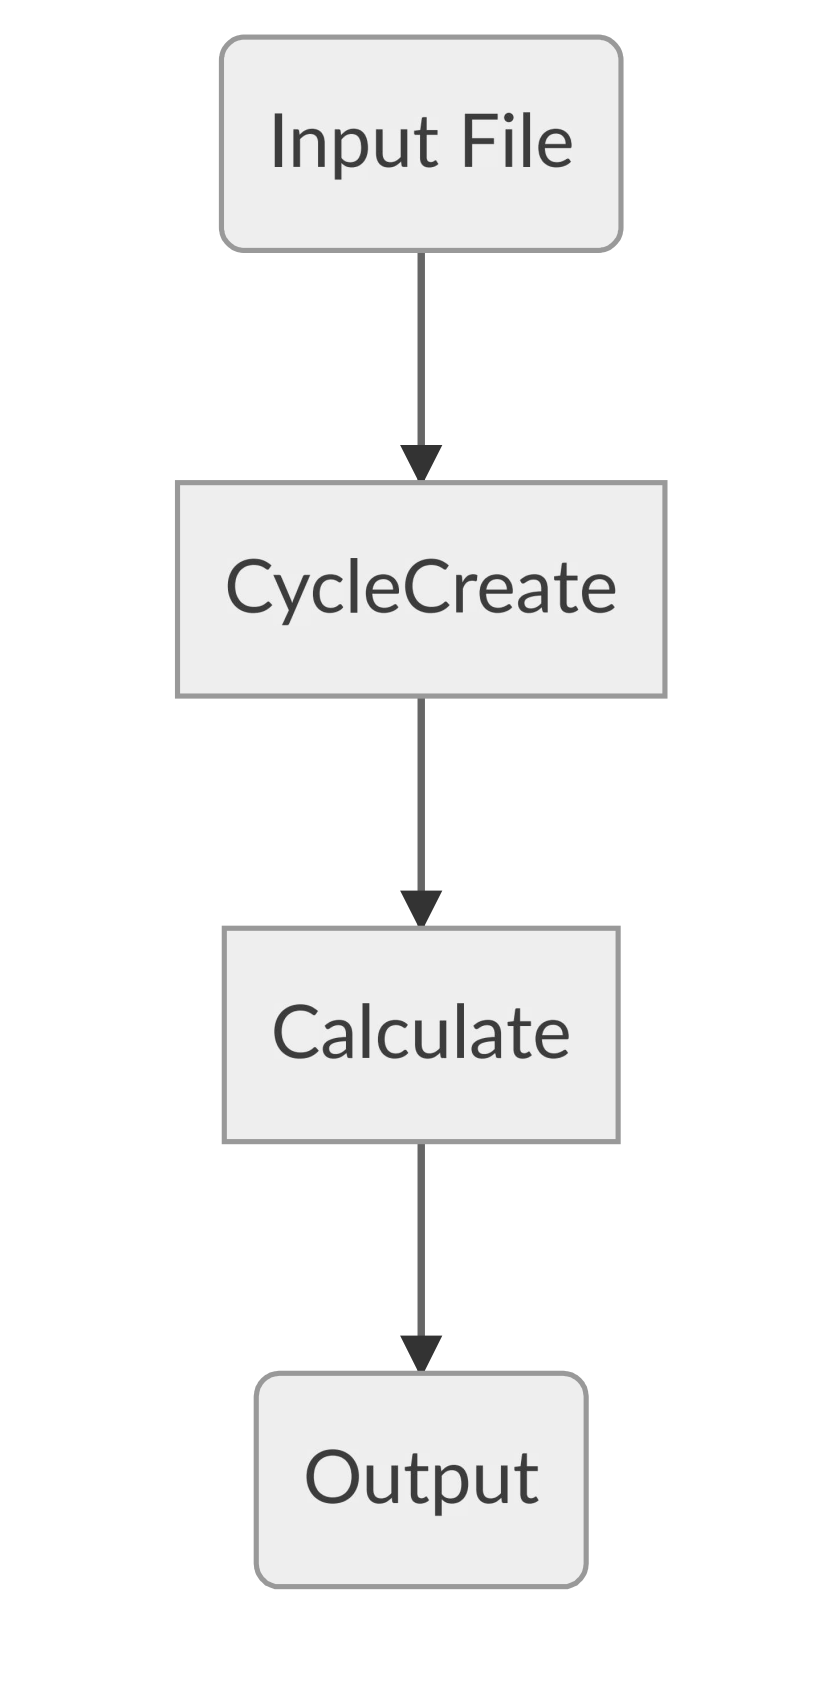
\includegraphics[width=0.2\textwidth]{Chapitre_6/Images/GeneralFlowChart.png}
\caption{General flow chart of the program}
\label{fig:C6_flowchart}
\end{figure}

Once provided, the program will first read the "Type" field to select the desired configuration. This is done by the function \textit{CycleCreate} that will create the model associated to the configuration selected. This function, for which the scheme is given in the Figure \ref{fig:C6_cyclecreate}, first parses the inputs file to extract the four dictionaries "Type", "Selection", "Input" and "Extra". 

\begin{figure}[h]
    \centering
    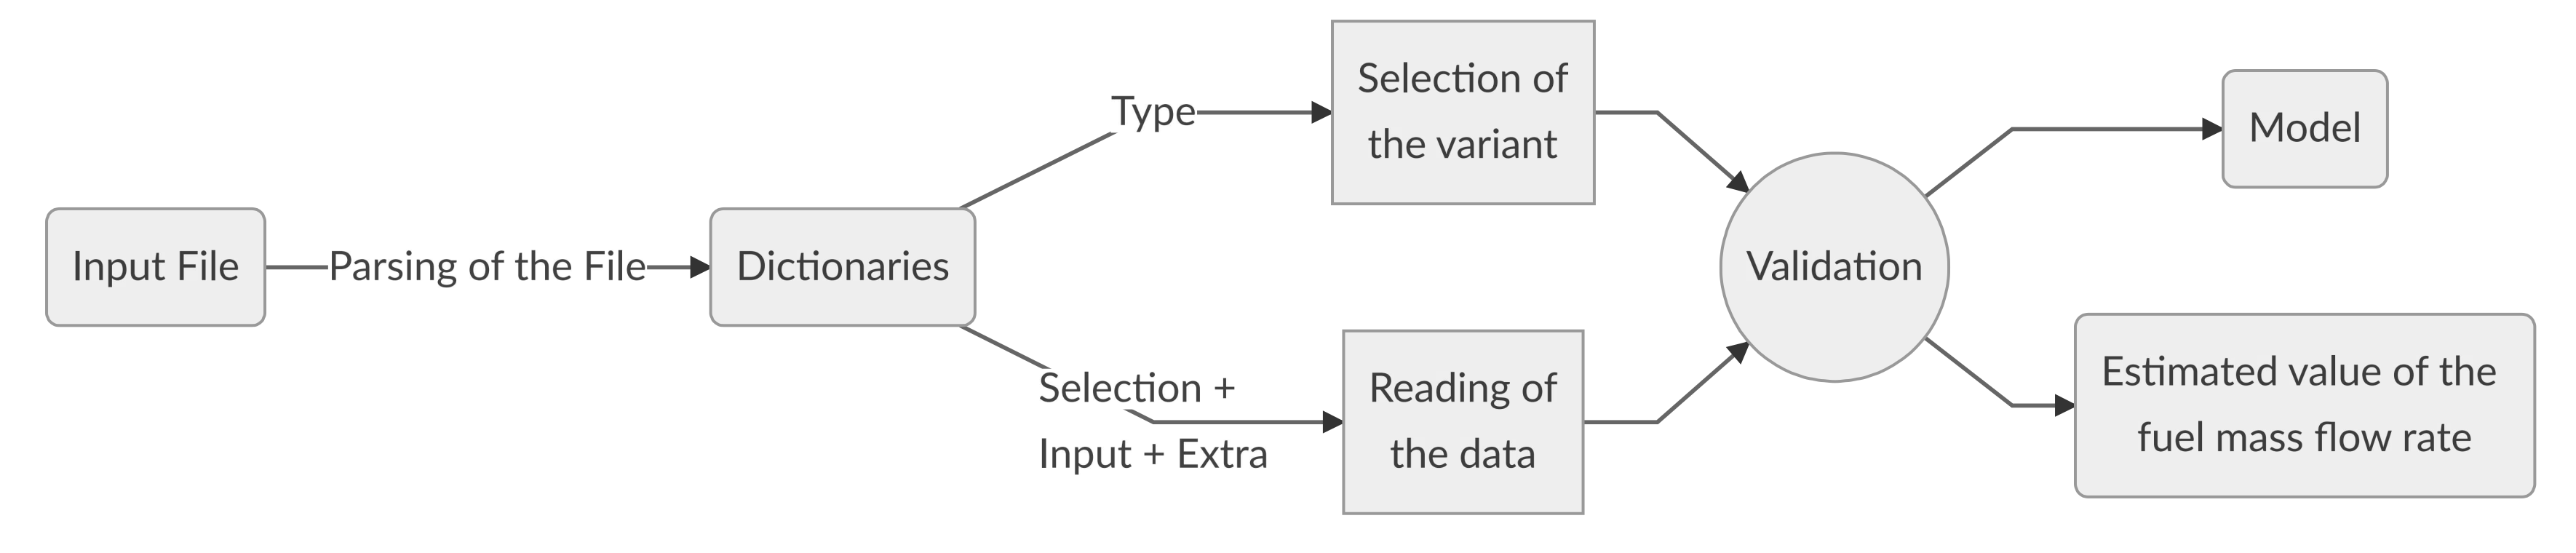
\includegraphics[width=0.9\textwidth]{Chapitre_6/Images/CycleCreate.png}
    \caption{Scheme of the function \textit{CycleCreate}}
    \label{fig:C6_cyclecreate}
\end{figure}
Then, all the data are read and stored. Based on the choice made in the "Selection" section, the function will search information in the dictionary named "Extra". 
Finally, the function validates the inputs read to ensure that the program will run without leading to an error induced by missing or wrong data. After this step of verification, the model for the selected configuration is created.

Once the model created, it is provided to the \textit{Calculate} function. The scheme of this function is provided in the Figure \ref{fig:C6_calculate}.

\begin{figure}[h]
    \centering
    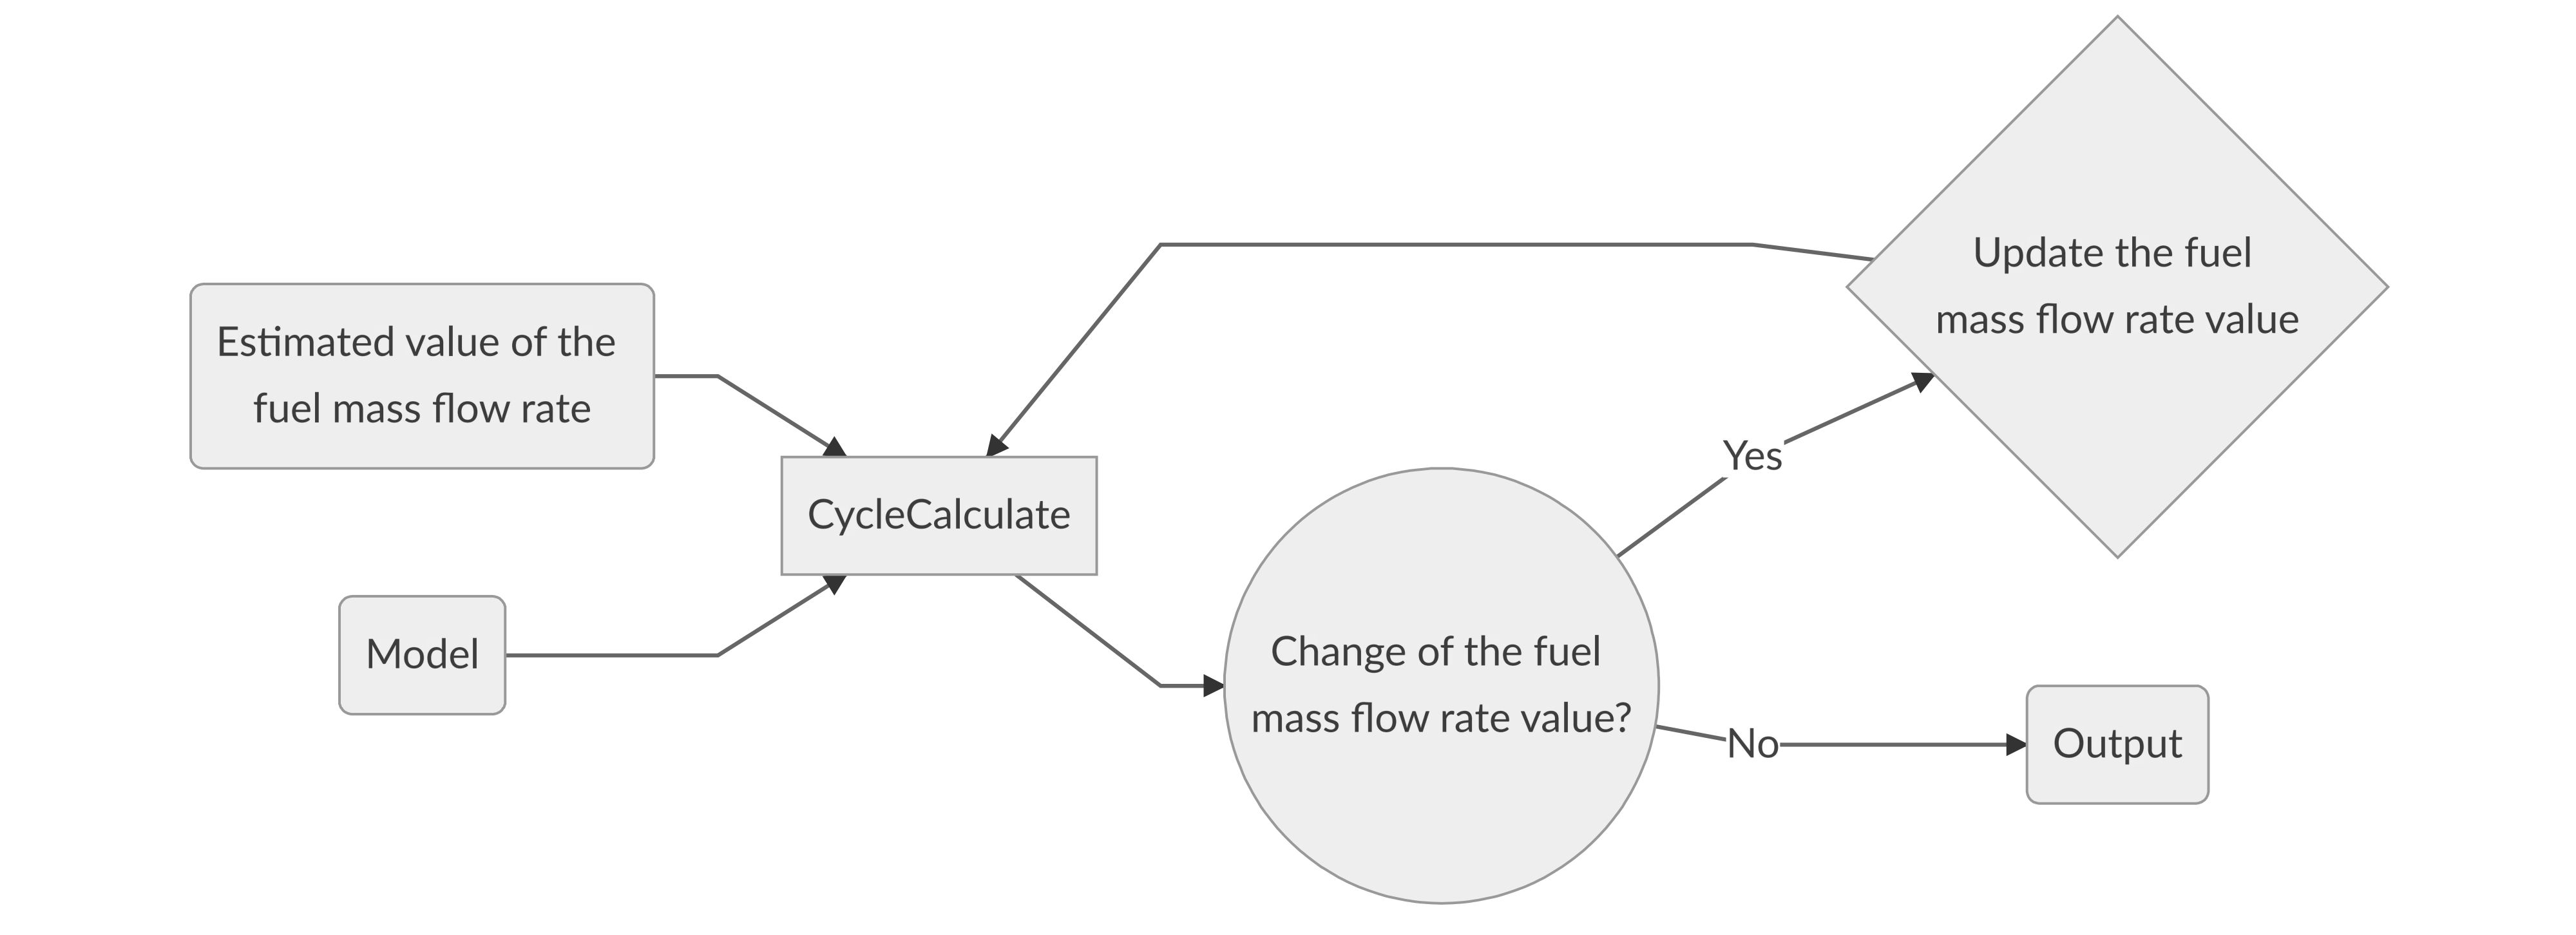
\includegraphics[width=0.9\textwidth]{Chapitre_6/Images/Calculate.png}
    \caption{Scheme of the function \textit{Calculate}}
    \label{fig:C6_calculate}
\end{figure}

Here, an initial guess for the mass flow rate of fuel injected into the combustion chamber is required. This guess value is obtained using the mass flow rate of air and the air factor $\lambda$. 

Then, the function \textit{CycleCalculate} is called. The structure of this function varies from one configuration to the other. Nevertheless, \textit{CycleCalculate} is a function that follows the path taken by the actual flow in the cycle. This function is composed of blocks (or objects) representing the elements constituting the cycle. Based the variant chosen, the order of these blocks will be different.  

Once the Brayton cycle completed, the value of the mass flow rate of fuel has been updated. If its value is different from the initial guess, the latter is updated and the function \textit{CycleCalculate} is called again. If the two values are really closed from one to the other, the program exits the loop and provides some outputs.

The outputs of the program are:

\begin{itemize}
\setstretch{1}
    \item The temperature, pressure, enthalpy, entropy and density for the defined states.
    \item The mass flow rate of fuel and the air factor.
    \item The power produced or consumed by the different elements.
    \item The efficiency of the different elements.
    \item The efficiency of the cycle.
    \item The corrected and reduced quantities associated to the turbomachines.
\end{itemize}

The interest of these outputs is to be able to quantify the performance of the cycle and to adapt some of the input in order to reach the desired results. For instance, for a gas turbine the target value for air factor is often in the neighboring of 8-10. Also, the TIT is in practice limited by the material constituting the turbine blades. Indeed, a large temperature would destroy the turbine by reaching the melting temperature of the material.

Next chapter will present the implementation method of each element constituting the cycle. For each of those, the functions involved will be defined and explained. Also, some links with the theoretical notions seen in chapters \ref{C2}, \ref{C3} and \ref{C4} will be created.






 